% This is samplepaper.tex, a sample chapter demonstrating the
% LLNCS macro package for Springer Computer Science proceedings;
% Version 2.21 of 2022/01/12
%
% \documentclass[runningheads]{llncs}
\documentclass[runningheads,dvipdfmx]{llncs}
%
\usepackage[T1]{fontenc}
% T1 fonts will be used to generate the final print and online PDFs,
% so please use T1 fonts in your manuscript whenever possible.
% Other font encondings may result in incorrect characters.
%
\usepackage{graphicx}
% Used for displaying a sample figure. If possible, figure files should
% be included in EPS format.
%
% If you use the hyperref package, please uncomment the following two lines
% to display URLs in blue roman font according to Springer's eBook style:
%\usepackage{color}
%\renewcommand\UrlFont{\color{blue}\rmfamily}
%\urlstyle{rm}
\usepackage{array}
\newcolumntype{C}[1]{>{\centering\arraybackslash}m{#1}}
\usepackage{multirow}
%
\begin{document}
%
\title{Vertical Split Encoding: Enabling Larger N-Tuples for Stronger 2048 Play}
%
%\titlerunning{Abbreviated paper title}
% If the paper title is too long for the running head, you can set
% an abbreviated paper title here
%
\author{Shunsuke Terauchi\inst{1} \and %\orcidID{0000-1111-2222-3333}
Kiminori Matsuzaki\inst{1}\orcidID{0009-0003-4663-3292}}
%
\authorrunning{S.~Terauchi and K.~Matsuzaki}
% First names are abbreviated in the running head.
% If there are more than two authors, 'et al.' is used.
%
\institute{Kochi University of Technology, Kam, Kochi 782--8502, Japan\\
\email{295141a@gs.kochi-tech.ac.jp}\\
\email{matsuzaki.Kiminori@kochi-tech.ac.jp}\\
}
%
\maketitle              % typeset the header of the contribution
%
\begin{abstract}
The abstract should briefly summarize the contents of the paper in
150--250 words.

\keywords{First keyword  \and Second keyword \and Another keyword.}
\end{abstract}
%
%
%
\section{Introduction}

N-tuple networks (a.k.a. pattern-based evaluation functions in Othello~\cite{Buro98}) are a simple but
efficient approach to designing evaluation functions for board games and other applications.
N-tuple networks compute an evaluation value by sampling local features on the board, retrieving the corresponding values from the lookup tables, and summing them up (or calculating a linear combination of them).
The parameters in the lookup tables are often adjusted by supervised learning or reinforcement learning techniques.
Several strong computer players have been developed based on N-tuple networks, for example,  for Othello~\cite{Buro98,Jask14,NgIL12,KuSM25}, \mbox{connect-4}~\cite{ThKK12}, connect-6~\cite{HuQP18}, EinStein W\"urfelt Nicht!~\cite{CHHH24,HsHs25}.

The target game in this study is \emph{2048}~\cite{2048}, a single-player stochastic game developed by G. Cirulli.
Several computer players have been implemented \cite{Mats21,ASOH22,GuCW22,SzJa14,YWHC16,Jask18,KGWW22,Zhou19,WaMa25}, among which the most successful approaches employ N-tuple networks as evaluation functions~\cite{SzJa14} in combination with Expectimax search~\cite{YWHC16}.
For instance, the state-of-the-art player developed by Guei et al.~\cite{GuCW22} achieved an average score of 625\,377 using two-stage N-tuple networks consisting of 8 $\times$ 6-tuples---trained by extended temporal-difference learning with optimistic initialization---, 6-ply Expectimax search, and a game-specific tile-downgrading technique.


In general, larger N-tuple networks yield better performance at the cost of larger memory sizes required and longer training times for tuning~\cite{TeMa25}.
Let N-tuple networks consist of $m$ $\times$ $n$-tuples, then we can consider two approaches to enlarging N-tuple networks.
The first approach is to increase the number $m$ of tuples.  Although this is relatively straightforward to implement, Oka and Matsuzaki~\cite{OkMa16} demonstrated that performance was saturated only with this approach.
The second approach is to increase the size $n$ of the tuples.  In the early stages of research on 2048, computer players improved performance by enlarging 4-tuples to 6-tuples~\cite{SzJa14,YWHC16}.  However, as Ja\'skowski~\cite{Jask18} suggested, further enlargement has been considered infeasible for game 2048 due to the exponential growth in the number of parameters.  Note that, in 2048, a board cell can take 18 possible values, and N-tuple networks with $m$\,$\times$\,$n$-tuples have $m\times 18^n$ parameters.  A 6-tuple network has $3.4\times 10^7$ parameters (requiring 13 GB of memory~\footnote{The memory size is calculated for the case that 8\,$\times$\,$n$-tuple networks with 2-stage, 64 bits per parameter, are tuned with temporal coherence learning~\cite{Jask18}.}), a 7-tuple network has $6.1\times 10^8$ parameters (235 GB), and an 8-tuple has $1.1\times 10^{10}$ parameters (4.2 TB).


In this study, we overcome the aforementioned limitation by proposing a novel encoding method, called \emph{Vertical Split Encoding} (\emph{VSE}). In $k$-VSE, we encode a board state into $k$ board instances based on the $k$ value ranges of interest. Here, for each value range, the encoded board instance takes fewer possible values by equating values outside the range (except for empty cells, represented as $E$).
For example, with 2-VSE with value ranges $2^1$--$2^8$ and $2^9$--$2^{17}$, a board $[E, 2^1, 2^{11}, 2^{12}, \ldots]$ is encoded in $[E, 2^1, L, L]$ and $[E, S, 2^{11}, 2^{12}]$, where $L$ and $S$ are newly introduced special labels denoting \emph{larger} and \emph{smaller} values, respectively.
With VSE, the number of parameters required for $m$\,$\times$\,$n$-tuples in 2048 is reduced to $m\times 11^n$ with 2-VSE, $m\times 9^n$ with 3-VSE, and $m\times 7^n$ with 4-VSE. The reduction is drastic: for example when $n=8$, the numbers of parameters are reduced to 3.9\% with 2-VSE, 1.2\% with 3-VSE, and 0.21\% with 4-VSE, respectively.


We demonstrate the effectiveness of VSE for 2048 with intensive experiments.
In addition to 6-tuple networks without VSE, we developed computer players using larger N-tuple networks: 7-tuple networks with 2-VSE, 8-tuple networks with 3-VSE, and even 9-tuple networks with 4-VSE.
All N-tuple networks are successfully trained on a commodity computer using at most 64 GB of memory, and the 7-, 8- and 9-tuple networks outperformed the 6-tuple baseline.
In particular, the best 8-tuple networks achieved an average score of 407\,206 with 1-ply lookahead (greedy) play, 547\,365 with 3-ply Expectimax search, and 587\,690 with 5-ply Expectimax search, which were significantly better than the 6-tuple baseline.

% 本研究の主な貢献は以下の2点である。
% 第一に,従来はメモリや学習時間の制約から現実的に扱うことが困難であった大規模タプルを実現可能とする,VSE を提案したことである.
% 第二に,VSEを用いた大規模Nタプルネットワークが,最先端プレイヤで用いられている6タプルベースのプレイヤを同一条件にて性能で上回ることを実験的に確認した点である。

% 本研究は,様々なゲームにおいて用いられているNタプルネットワークにおいてパラメータを削減する新しい方法を提案するものである.

The main contributions of this study are twofold.
\begin{itemize}
 \item We proposed Vertical Split Encoding (VSE) to enable the employing of large $N$-tuple networks, which had been impractical due to memory constraints.
 \item We experimentally demonstrated that large N-tuple networks with VSE outperformed the 6-tuple baseline in the same experimental setting.
\end{itemize}
More broadly, this work introduces a novel approach for reducing parameters in N-tuple networks, which would be widely applied across various games.

% LocalWords:  EinStein urfelt Nicht Cirulli Guei et al expectimax Oka
% LocalWords:  Ja skowski VSE lookahead

\section{Game 2048}

2048 is a single-player stochastic game played on a $4 \times 4$ grid.
The objective of the original game is to reach a 2048-tile by moving and merging
the tiles on the board according to the rules below.
In an initial state, two tiles are placed randomly each with a number 2 (with probability $0.9$) or 4 (with probability $0.1$).
The player selects a direction (either up, right, down, or left), and then all the tiles will move in the selected direction.
When two tiles of the same number collide, they create a tile with the sum value and the player gets the sum as the score.
The merges occur from the far side and newly created tiles do not merge again on the same move: move to the right from \verb*|222 |, \verb*| 422| and \verb*|2222| results in
\verb*|  24|, \verb*|  44|, and \verb*|  44|, respectively.
Note that the player cannot select a direction in which no tiles move nor merge.
After each move, a new tile appears randomly at an empty cell with a number 2 (with probability $0.9$) or 4 (with probability $0.1$).
If the player cannot move the tiles in any direction, the game ends.

Fig.~\ref{fig:states-and-afterstates} depicts the process of the game.
Selecting right at the state $s_t$ in Fig.~\ref{fig:states-and-afterstates}, the tiles move to the right and
two 2-tiles and two 8-tiles merge adding the score 4 + 16 = 20.
Then, a new tile appears to reach the next state $s_{t+1}$.

\begin{figure}
  \centering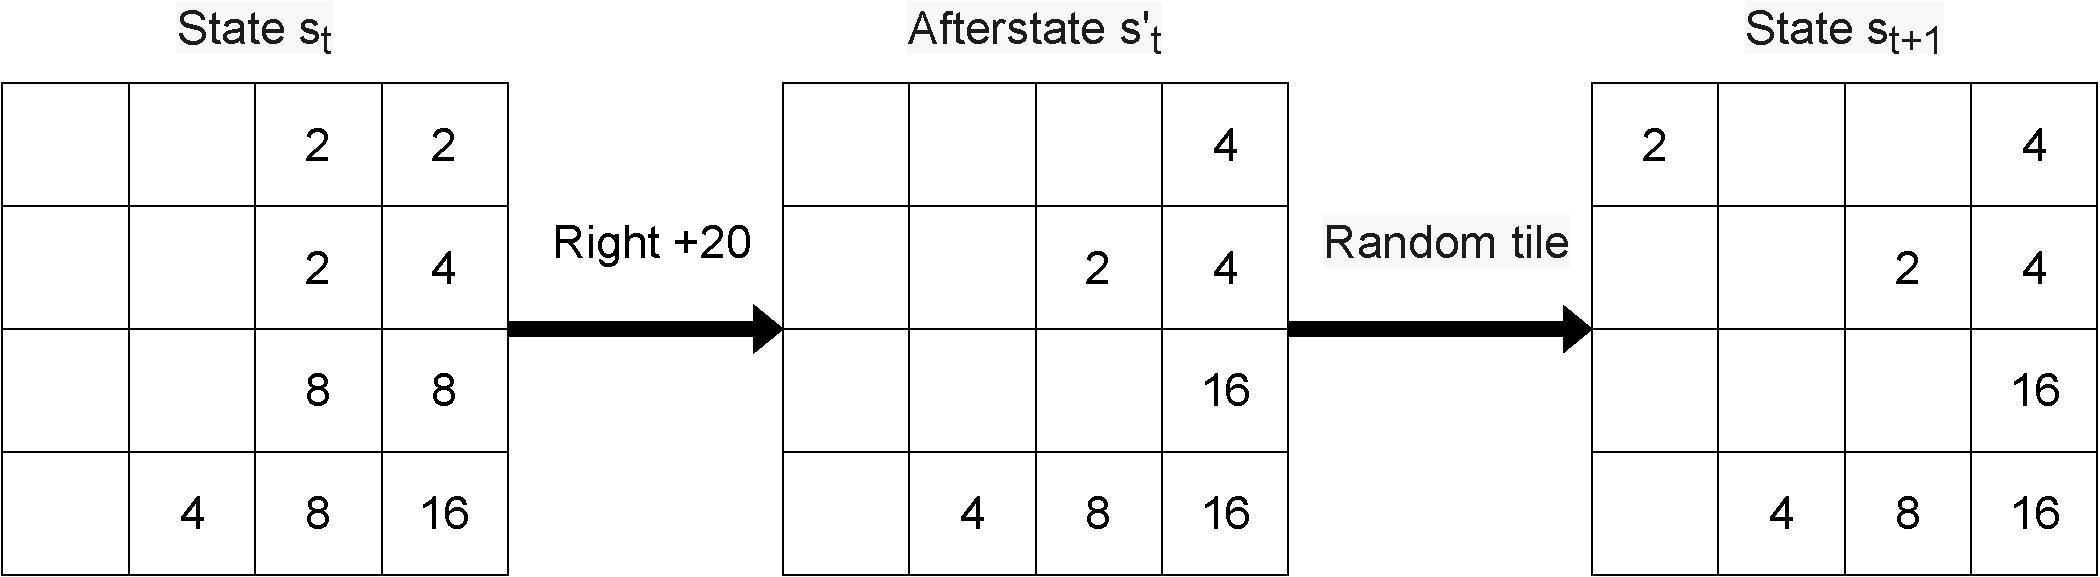
\includegraphics[width=.8\linewidth]{figures/state_afterstate.pdf}
 \caption{Process of game 2048}
 \label{fig:states-and-afterstates}
\end{figure}

Since a turn in 2048 consists of two steps, we introduce the two notions, called \emph{state} and \emph{afterstate}~\cite{SzJa14}, as shown in Fig.~\ref{fig:states-and-afterstates}.
\begin{itemize}
 \item A \emph{state} $s_t$ is a board (and score) at which the player selects a move.
 \item An \emph{afterstate} $s'_t$ is a board (and score) after the slide-and-merge step and before a new tile appears.
\end{itemize}

For better understanding of the performance of the players, Table~\ref{table:achievement} summarizes the common score achieved and the common number of moves needed when the player reaches a tile of a specific value.

\begin{table}
 \caption{Score and number of moves when a tile is first created}
\setlength{\doublerulesep}{.4pt}
 \label{table:achievement}
 \centering\begin{tabular}{lrrrrr}
\hline
\hline
  tile & \makebox[4em][r]{2048} & \makebox[4em][r]{4096} & \makebox[4em][r]{8192} & \makebox[4em][r]{16384} & \makebox[4em][r]{32768} \\
\hline
  score & 20\,000 & 44\,000 & 97\,000 & 210\,000 & 450\,000 \\
\hline
  moves &     950 & 1\,900 &  3\,800 & 7\,600 & 15\,200 \\
\hline
 \end{tabular}
\end{table}

% 図\ref{afterstate2048}は,初期局面から始まるゲームの流れにおいて,state,afterstate,progress を図示したものである.


\section{Vertical Split Encoding for N-tuple Networks}

% 2048 の強いコンピュータプレイヤを作る最も成功した方法は,N タプルネットワークによる評価関数を強化学習によりチューニングするものである。Nタプルネットワークは,盤面の (局所的な) サンプリングとlook-up tableによる評価関数の近似関数である.各N-tupleに対して該当する場所の値をサンプリング・look-up tableから局所評価値を取得し,それら局所評価値を足し合わせることで全体の評価関数を得る.2048では,盤面の対称性から,一つのNタプルに対して8通りのサンプリングを行うことが一般的であり,本研究でもその対称性の利用を採用する.
The most successful approach to building a strong computer player for 2048 is to use an evaluation function based on N-tuple networks, whose parameters are tuned through reinforcement learning.
N-tuple networks are function approximators implemented with (local) sampling of the board and the corresponding lookup tables.
For each N-tuple (examples of N-tuples are given in Fig.~\ref{fig:NTupleVSE}), we sample a set of cells corresponding to the tuple elements, retrieve the corresponding values from the lookup table, and sum these values up to compute the overall evaluation value.
A common practice in 2048 is to perform eight-fold sampling for each N-tuple by exploiting board symmetries~\cite{SzJa14}, and does our study.

Increasing the size of the tuples is expected to yield significant performance improvements.
Oka and Matsuzaki~\cite{OkMa16} investigated the use of 6- and 7-tuples, showing that the use of 7-tuples achieved superior performance. We also confirmed for mini2048 (a $3\times 3$ variant of 2048) that increasing the size of N-tuples yielded a performance improvement of up to 6-tuples~\cite{TeMa25}.

% ニューラルネットワークと比べて,Nタプルネットワークは高速に評価値を計算することができるものの,一般に必要となるメモリ量が多い.盤面の各セルのとりうる値が $x$ 種類,タプルの数が m,タプルの大きさが n であるとき,look-up table は $m \times x^n$ 要素からなる.2048では,$\mbox{empty}, 2^1, 2^2, \ldots, 2^17$ の$x=18$通りの値をとりうるため,$n$ を増やしたときに必要となるメモリが問題となってしまう.実際,Jaskowski は,(multi-staging を採用できない)7タプルに拡大するよりも,6タプルとmulti-staging を組合せることが有用だと実験で示した.
However, N-tuple networks require a large amount of memory.
When we consider $m$ tuples of size $n$ and each cell on the board can have one of $x$ distinct values, a lookup table consists of $m \times x^n$ entries.
In 2048, since the number of possible cell values is 18 ($\mbox{empty}, 2^1, 2^2, \ldots, 2^{17}$), the memory requirement becomes an issue as $n$ increases.
Table~\ref{table:NTupleMemory} summarizes the number of parameters required in a lookup table for a single $n$-tuple and for eight $n$-tuples, when $n$ is between 6 and 9, as well as the memory usage when combining the currently dominant methods of multi-staging~\cite{YWHC16} and Temporal Coherence learning~\cite{Jask18}.
In practice, it has been believed that 7-tuples or larger could not work on commodity computers (e.g., within 64 GB of memory).
Indeed, Ja\'skowski~\cite{Jask18} experimentally demonstrated that it was more effective to use 6-tuples in combination with the multi-staging technique, rather than using a single 7-tuple without multi-staging.

% しかしながら,タプルサイズを増やすことができれば,大きな性能向上が見込まれる.Matsuzaki は,6タプルと7タプルの組合せとプレイヤの性能の関係を調べ,7タプルのほうが性能が優れていた.しかし,上述のメモリサイズの問題が発生する.
% Nタプルの大きさを 6~9 としたとき,1つのN-tuple に対してlook-up テーブルに必要となるパラメータ数,現在主流となっている Multi-staging と Temoral Coherence 学習を組み合わせた場合のメモリ量を表\ref{table:NTupleMemory}にまとめる.
% 一般は,4個以上のN-tuple を組み合わせて用いるので,commodity computer (e.g. computer with 64GB メモリ) では 7-tuple 以上を実現することができないと考えられていた.
\begin{table}
\setlength{\doublerulesep}{.4pt}
 \caption{Number of parameters and required memory size.  In the calculation of memory size, we assume an implementation of temporal coherence learning with 2 stages and 64 bits per element.}
\label{table:NTupleMemory}
 \centering\begin{tabular}{l|rr||l|rr}
\hline\hline
  \multicolumn{1}{c|}{network} & \multicolumn{1}{c}{parameters} & \multicolumn{1}{c||}{memory} & \multicolumn{1}{c|}{network} & \multicolumn{1}{c}{parameters} & \multicolumn{1}{c}{memory} \\
\hline
  $1 \times 6$-tuple & 34\,012\,224 & 1.5 GB &  $8 \times 6$-tuple & 272\,097\,792 & 12.2 GB \\
  $1 \times 7$-tuple & 612\,220\,032 & 27.4 GB &  $8 \times 7$-tuple & 4\,897\,760\,256 & ~~218.9 GB \\
  $1 \times 8$-tuple & 11\,019\,960\,576 & ~~492.6 GB &  $8 \times 8$-tuple & 88\,159\,684\,608 & 3.9 TB \\
  $1 \times 9$-tuple & 198\,359\,290\,368 & 8.9 TB &  $8 \times 9$-tuple & 1\,586\,874\,322\,944 & 70.9 TB \\
\hline
% (*    18 18 18 18 18 18 18 18 18 8)
% (/ (* 18 18 18 18 18 18 18 18 18 8 8 3 2) 1024.0 1024.0 1024.0)
 \end{tabular}
\end{table}

% このメモリサイズの問題を解決し,大規模タプルを効率的に扱うための新手法として,本研究では Vertical Split Encoding (VSE) を提案する.上述のとおり,メモリサイズがとても大きくなる理由は,盤面の取り得る値の種類 $x=18$ が大きいからである.一方で,著者らは2048における次の特徴に着目した.
% - 値の近いタイルの間の位置関係は重要である
% - 値の遠いタイルは相互作用しない
% - 空白マスの位置は重要である.
% これらの特徴のうち,2つ目の特徴から,ある値のタイルに着目すると,それと値が大きく離れたタイルは区別する必要がないことを示唆する.例えば,値が 2 (= $2^1$) のタイルに着目すると,その周辺にある値 $2048 = 2^{11}$ や $4096 = 2^{12}$ を区別するのはほとんど意味をなささい.したがって,そのような値が大きく離れたタイルを同一視することで,パラメータ数を減らすことができると考えた.

To address the issue of memory requirement and hence to enable large N-tuple networks, this study proposes a novel method called \emph{Vertical Split Encoding} (VSE)~\footnote{The idea behind the term ``Vertical'': the input space of 2048 is in three dimensions, the first two are for the position on a board, and the third is for the cell values. Vertical Split Encoding works on this third dimension.}.
As noted above, the main reason for the huge memory requirement is that the number of possible cell values on the board is large, $x = 18$.
Here, we notice the following characteristics of 2048.
\begin{itemize}
 \item The relative positions of tiles with \emph{similar} values are important.
 \item Tiles with \emph{widely different} values do not interact.
 \item The positions of empty cells are important.
\end{itemize}
Among these, the second characteristic suggests that, when looking at a particular tile value, it is unnecessary to distinguish tiles whose values are very far apart. For example, when looking at a tile of value $2^1$, distinguishing whether the neighboring tiles are $2^{11}$ or $2^{12}$ is almost meaningless.
Therefore, by equating tiles with widely different values, we can reduce the number of possible values and accordingly the number of parameters in the lookup tables.

% この考えに基づき,Vertical Split Encoding は,盤面を,いくつかの値を同一視した複数の盤面にエンコードする.
% 各エンコードでは,着目したい値の範囲を value range とし,その範囲より小さい・大きい値はすべて S・L に置き換える.
% ただし,上で述べた2048の特徴の3より,empty cell (E) については特別扱いする.
% 図に具体例を示す.ここでは,value ranges は 1--10 と 11-17 とする.
% このとき,一つ目のエンコードでは,$2^{11}$~$2^{17}$の値を持つタイルはすべて L となり,2つ目のエンコードでは
% $2^{1}$~$2^{10}$ のタイルはすべて S となる.これにより,1つ目のエンコードについては,各セルのとりうる値が $x_1 = 1 + 10 + 1 = 12$ 通り,2つ目のエンコーディングでは $x_2 = 1 + 1 + 7 = 9$ 通りとなり,look-up table の要素数を大きく減少させられる.
Based on this idea, Vertical Split Encoding maps a board into multiple board instances, in each of which some board cells have the same label.
First, we define a set of \emph{value ranges} of interest: All values smaller than this range are replaced by $S$, and all the larger values are replaced by $L$.
To address the third characteristic mentioned above, we treat empty cells (E) separately.

A concrete example is shown in Fig.~\ref{fig:VSE-example}, where value ranges of interest are $2^1$--$2^8$ and $2^9$--$2^{17}$.
In the first mapping, all tiles with values larger than $2^{8}$ are replaced by $L$.
In the second mapping, all the tiles with values smaller than $2^{9}$ are replaced by $S$.
After these mappings, the resulting possible values are $[{E}, 2^1, 2^2, 2^3, 2^4, 2^5, 2^6, 2^7, 2^8, {L}]$ in the first mapping and $[{E}, {S}, 2^9, 2^{10}, 2^{11}, 2^{12}, $\break$2^{13}, 2^{14}, 2^{15}, 2^{16}, 2^{17}]$ in the second mapping.
As a result, the numbers of possible values are $x_1 = 10$ and $x_2 = 11$, respectively, which significantly reduces the memory requirement for the lookup tables.

\begin{figure}
 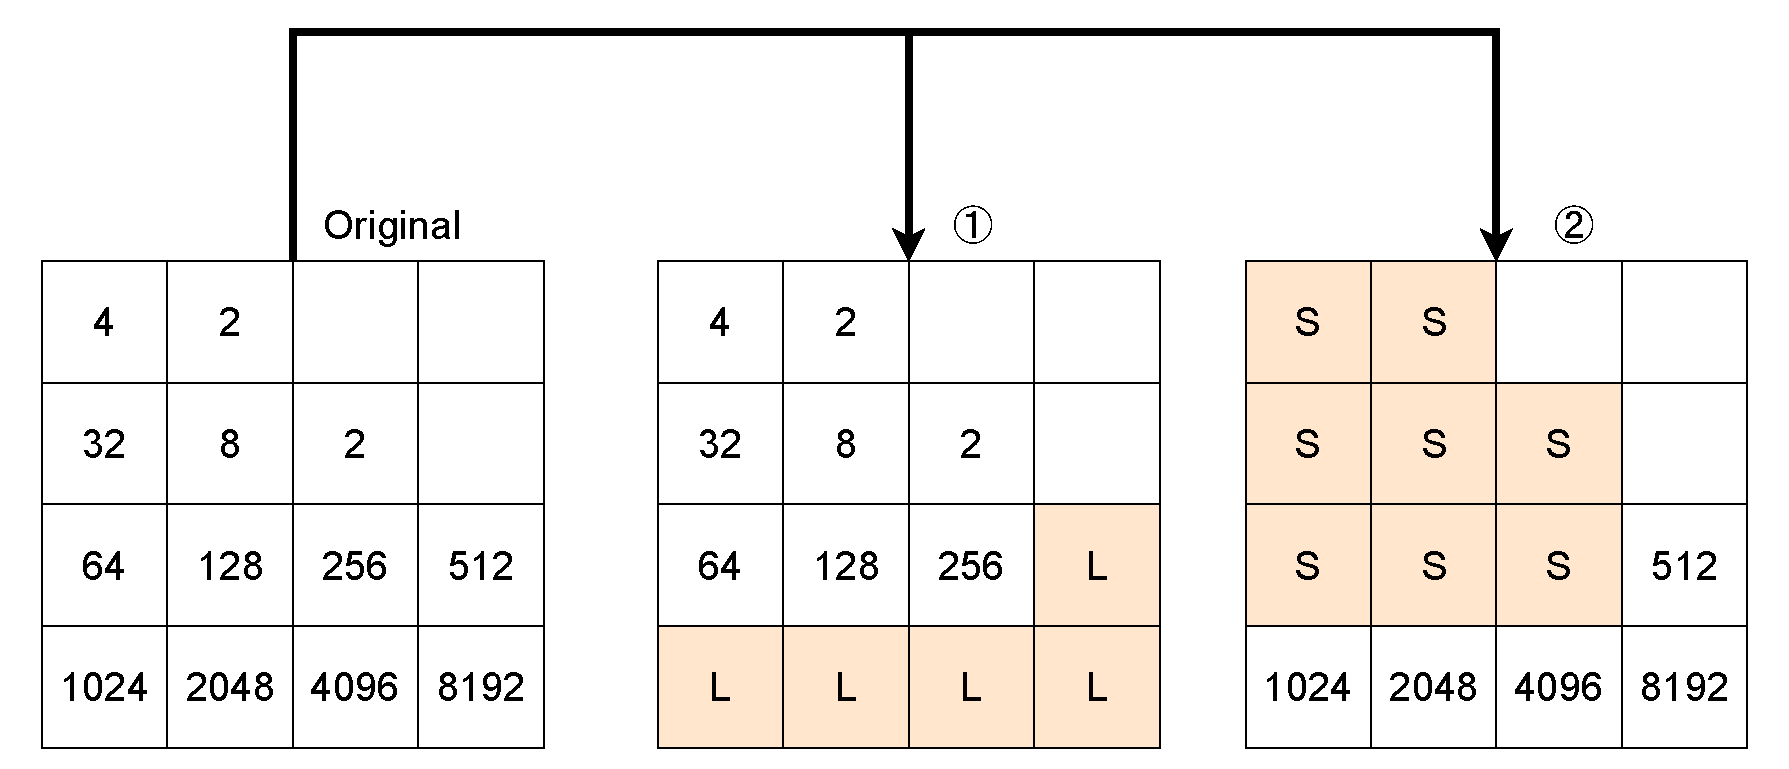
\includegraphics[width=.9\linewidth]{figures/VSE-example.pdf}
 \caption{An example of Vertical Split Encoding with two value ranges 1--8 and 9--17.}
 \label{fig:VSE-example}
\end{figure}

% 後述する2048に対する実験では,7タプル,8タプル,9タプルに対し,それぞれ,2つ,3つ,4つのvalue ranges からなるVSEを適用し,プレイヤの性能を評価する.

We can extend the idea to $k$-VSE, with $k$ value ranges of interest.
In the experiments on 2048 described later, we apply 2-, 3-, and 4-VSE.

% LocalWords:  approximators Ja skowski VSE

\section{Preliminary Experiments on Mini2048}

% VSE を行うことで性能がどのくらい下がりうるのか,どのように value ranges を設計すればよいかについて
% 知見を得るため,まず 3x3 の mini2048 を用いて評価を行った.
% mini2048 は,3x3 の盤面で行われること以外は2048と同じである.
% すでに完全解析されており,理論的な最高期待値は5469?点だと分かっている.
% 著者らの先行研究において,様々な大きさのN-tupleを設計・実験し,盤面の半分以上をカバーする7タプルまで性能向上が見られることを示した.

We first conducted evaluations of VSE using mini2048, a smaller variant of 2048, to gain insights of how much the application of VSE degrates the performance and of which proporties of value ranges affect the preformance.
Mini2048 is a smaller variant of 2048 where the game rules are identical to 2048 except for the board size being $3\times 3$.
We chose Mini2048 as the testbed of our preliminary experiments for two reasons: it was strongly solved (a.k.a. perfectly analized) and the expected score of the optimal play is known to be 5469; we confirmed in our previous work that enlarging the size of N-tuple yielded better performance up to 6-tuples (each 6-tuple samples from two-thirds of the board).

% 実験では,m-NT6 を例にとり,複数の value ranges の組合せによる VSE を行ったときのプレイヤの性能を調べる.
% ここでは,最大3つに分割する VSE を複数試す.ここで調べたいことは以下の3つである.
%  - VSE を行うことで,どのくらいの性能低下がありうるか.
%  - 分割にあたって,複数の分割に含まれるバッファを持たせるべきか.
%  - VSE を行ったときに,性能に最も影響する要素は何か.

In the preliminary experiments, we used two manually designed N-tuple networks in Table~\ref{table:mNT}: two 6-tuples (namely, \textsf{mNT6}) and three 4-tuples (namely, \textsf{mNT4}). For \textsf{mNT6}, we applied multiple VSEs that split the value ranges up to three parts.
The main questions we wished to examine were the following:
\begin{itemize}
 \item To what extent does VSE degrade the performance?
 \item Should we have operlaps between value ranges when splitting?
 \item Which factor of VSE affects the performance most strongly?
\end{itemize}


% 比較として,VSE を行わない m-NT4 の結果も示す.
% 学習は,OI=1200 で初期化したTC学習とし,$5\times10^8$ steps だけ学習させる.
% 10個の異なるseedsを用いた学習から得られる10個のプレイヤにgreedy に??ゲームプレイさせたときの平均得点を調べる.

For each configuration, we trained N-tuple networks using Temporal Coherence learning with optmistic initialization (initial value 1200) for $5\times 10^8$ steps.  After the training, we played 1000?? games with 1-ply lookahead (the greedy play), and evaluate the performance in terms of the average score.  To mitigate the effect of randomness, we conducted each training with 10 different random seeds.
Table~\ref{table:pre-results} summarizes the configuratons of VSE and the average score of the trained N-tuple networks.

\begin{table}
 \caption{N-tuple networks used for mini2048.}
 \label{table:mNT}
 \centering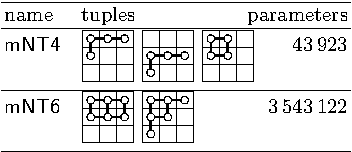
\includegraphics[]{figures/mNT-table.pdf}
\end{table}

\begin{table}
\caption{Configurations of preliminary experiments for mini2048 and the average score for 1000 games with 1-ply lookahead (the numbers after $\pm$ show standard deviation over 10 training runs).}
\label{table:pre-results}
 \setlength{\doublerulesep}{.4pt}
 \small\begin{tabular}{l|l|p{170pt}|r|r}
  \hline\hline
   tuple			& VSE			& value ranges									& weights	& ave. score \\
  \hline
% (* 11 11 11 11 11 11 1 2)3543122
   \multirow{11}{*}{mNT6}	& \mbox{no VSE}		& \phantom{\rule{1pt}{9.5pt}}$2^1$--$2^{10}$ (11)								& 3\,543\,122	& 4\,610.2$\pm$\phantom{0}81.1 \\ \cline{2-5}
% (* 8 8 8 8 8 8 2 2)1048576
				& \mbox{2-VSE-A}	& \phantom{\rule{1pt}{9.5pt}}$2^1$--$2^6$ (8), $2^{5}$--$2^{10}$ (8)					& 1\,048\,576	& 4\,555.8$\pm$\phantom{0}91.7\\ \cline{2-5}
% (+ (* 8 8 8 8 8 8 1 2) (* 7 7 7 7 7 7 1 2))759586
				& \mbox{2-VSE-B}	& \phantom{\rule{1pt}{9.5pt}}$2^1$--$2^6$ (8), $2^{6}$--$2^{10}$ (7)					& 759\,586	& 4\,584.0$\pm$\phantom{0}69.9\\ \cline{2-5}
% (+ (* 8 8 8 8 8 8 1 2) (* 6 6 6 6 6 6 1 2))617600
				& \mbox{2-VSE-C}	& \phantom{\rule{1pt}{9.5pt}}$2^1$--$2^6$ (8), $2^{7}$--$2^{10}$ (6)					& 617\,600	& 4\,557.3$\pm$\phantom{0}74.5\\ \cline{2-5}
% (+ (* 7 7 7 7 7 7 2 2))470596
				& \mbox{2-VSE-D}	& \phantom{\rule{1pt}{9.5pt}}$2^1$--$2^5$ (7), $2^{6}$--$2^{10}$ (7)					& 470\,596	& 4\,621.1$\pm$\phantom{0}83.5\\ \cline{2-5}
% (+ (* 6 6 6 6 6 6 1 2) (* 8 8 8 8 8 8 1 2))617600
				& \mbox{2-VSE-E}	& \phantom{\rule{1pt}{9.5pt}}$2^1$--$2^4$ (6), $2^{5}$--$2^{10}$ (8)					& 617\,600	& 4\,441.4$\pm$\phantom{0}96.7\\ \cline{2-5}
% (+ (* 6 6 6 6 6 6 2 2) (* 5 5 5 5 5 5 1 2))217874
				& \mbox{3-VSE-A}	& \phantom{\rule{1pt}{9.5pt}}$2^1$--$2^4$ (6), $2^{5}$--$2^{7}$ (6), $2^8$--$2^{10}$ (5)			& 217\,874	& 4\,390.9$\pm$111.6\\ \cline{2-5}
% (+ (* 6 6 6 6 6 6 2 2) (* 7 7 7 7 7 7 1 2))
				& \mbox{3-VSE-B}	& \phantom{\rule{1pt}{9.5pt}}$2^1$--$2^4$ (6), $2^{4}$--$2^{7}$ (7), $2^7$--$2^{10}$ (6)			& 421\,922	& 4\,464.9$\pm$\phantom{0}64.7\\ \cline{2-5}
% (+ (* 6 6 6 6 6 6 1 2) (* 5 5 5 5 5 5 2 2) (+ 4 4 4 4 4 4 1 2))155839
				& \mbox{4-VSE-A}	& \phantom{\rule{1pt}{9.5pt}}$2^1$--$2^4$ (6), $2^5$--$2^6$ (5), $2^7$--$2^8$ (5), $2^9$--$2^{10}$ (4)	& 155\,839	& 4\,451.7$\pm$\phantom{0}96.7\\ \hline
   mNT4				& \mbox{no VSE}		& \phantom{\rule{1pt}{9.5pt}}$2^1$--$2^{10}$ (11)								& 43\,923	& 3\,226.0$\pm$141.4\\\hline
 \end{tabular}
\end{table}

% 表より,とても promissing な結果が得られた.
% VSE を行うことで,性能低下は起こりうるが,m-NT4 との比較からタプルサイズ拡大による性能向上を打ち消すほどではない.
% 分割の際に,複数の分割に共通の値が含まれるようなバッファを用いる必要はない.
% これは,著者らの当初の想定に反する結果であった.
% 性能に最も影響するのは,一番小さなrangeに含まれる要素数である.
% 一番小さな range に含まれる要素数が同じであれば,それより上のrangeをさらに分割してもしなくても大差ないようだ.

The results in Table~\ref{table:pre-results} were highly promising.
All the results from \textsf{mNT6} plus VSEs outperformed that of \textsf{mNT4}.
While applying VSE degrate the performance (for the case of mNT6, $<$5\%) in general, the N-tuple networks by 2-VSE-D was slightly better than the original mNT6.
From the results of 2-VSE-A, 2-VSE-B, and 2-VSE-C as well as 3-VSE-A and 3-VSE-B, it is not necessary to introduce overlaps between value ranges---this was contrary to the authors' initial assumption.
The factor with the greatest impact on performance is the number of elements included in the smallest value range as seen in 2-VSE-C, 2-VSE-D, and 2-VSE-E
If the size of the smallest range is the same, then further splitting of higher ranges appears to make little difference as seen in 2-VSE-E, 3-VSE-A, and 4-VSE-A.

We will use these findings in the design of VSEs for original 2048.

\begin{table}
 \begin{tabular}{|C{15pt}|C{15pt}|C{15pt}|C{15pt}|C{15pt}|C{15pt}|C{15pt}|C{15pt}|C{15pt}|C{15pt}|C{15pt}|C{15pt}|C{15pt}|C{15pt}|C{15pt}|C{15pt}|C{15pt}|C{15pt}|}
  \multicolumn{18}{l}{(a) 1 layer with 18 elements}\\\hline
   0 & 1 & 2 & 3 & 4 & 5 & 6 & 7 & 8 & 9 & 10 & 11 & 12 & 13 & 14 & 15 & 16 & 17 \\\hline
  \multicolumn{18}{l}{}\\
  \multicolumn{18}{l}{(b) 2 layers with $11 + 10$ elements}\\\hline
   0 & 1 & 2 & 3 & 4 & 5 & 6 & 7 & 8 & 9 & \multicolumn{8}{c|}{$10 \le x$} \\\hline
   0 & \multicolumn{9}{c|}{$1 \le x \le 9$} & 10 & 11 & 12 & 13 & 14 & 15 & 16 & 17 \\\hline
  \multicolumn{18}{l}{}\\
  \multicolumn{18}{l}{(b) 3 layers with $9 + 9 + 6$ elements}\\\hline
   0 & 1 & 2 & 3 & 4 & 5 & 6 & 7 & \multicolumn{10}{c|}{$8 \le x$} \\\hline
   0 & \multicolumn{7}{c|}{$1 \le x \le 7$} & 8 & 9 & 10 & 11 & 12 & 13 & \multicolumn{4}{c|}{$14 \le x$}\\\hline
   0 & \multicolumn{13}{c|}{$1 \le x \le 13$} & 14 & 15 & 16 & 17 \\\hline
  \multicolumn{18}{l}{}\\
  \multicolumn{18}{l}{(b) 4 layers with $7 + 7 + 7 + 6$ elements}\\\hline
   0 & 1 & 2 & 3 & 4 & 5 & \multicolumn{12}{c|}{$6 \le x$} \\\hline
   0 & \multicolumn{5}{c|}{$1 \le x \le 5$} & 6 & 7 & 8 & 9 & \multicolumn{8}{c|}{$10 \le x$}\\\hline
   0 & \multicolumn{9}{c|}{$1 \le x \le 9$} & 10 & 11 & 12 & 13 & \multicolumn{4}{c|}{$14 \le x$}\\\hline
   0 & \multicolumn{13}{c|}{$1 \le x \le 13$} & 14 & 15 & 16 & 17 \\\hline
 \end{tabular}
\end{table}

\begin{table}
 \setlength{\doublerulesep}{.4pt}
\begin{tabular}{p{1.2cm}l@{~~}r}
  \hline\hline
  name & tuples & parameters \\\hline
\raisebox{15pt}{\textsf{NT6-M}}
&
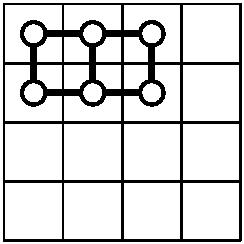
\includegraphics[width=0.9cm]{figures/NTuple-0.pdf}
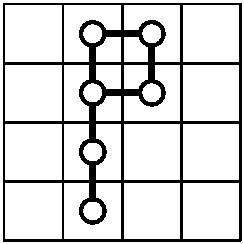
\includegraphics[width=0.9cm]{figures/NTuple-1.pdf}
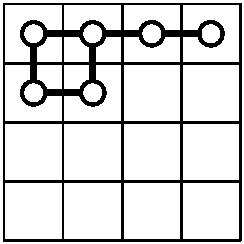
\includegraphics[width=0.9cm]{figures/NTuple-2.pdf}
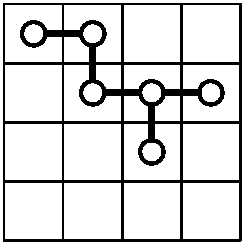
\includegraphics[width=0.9cm]{figures/NTuple-3.pdf}
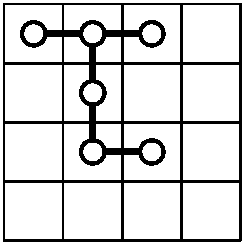
\includegraphics[width=0.9cm]{figures/NTuple-4.pdf}
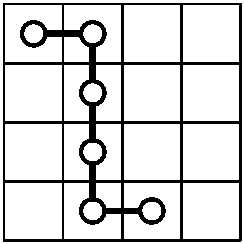
\includegraphics[width=0.9cm]{figures/NTuple-5.pdf}
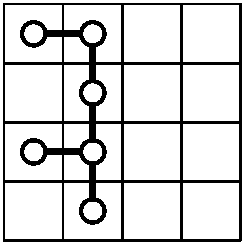
\includegraphics[width=0.9cm]{figures/NTuple-6.pdf}
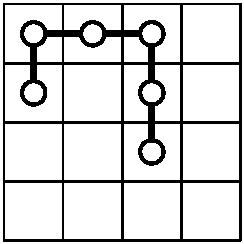
\includegraphics[width=0.9cm]{figures/NTuple-7.pdf}
& \raisebox{10pt}{$\begin{array}{r}
 \mbox{1 board, 2 stages}\\
544\,195\,584
 \end{array}$}
\\\hline
\raisebox{15pt}{\textsf{NT6}}
& 
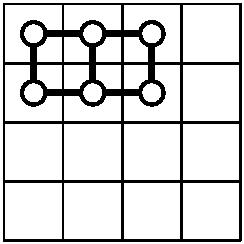
\includegraphics[width=0.9cm]{figures/NTuple-60.pdf}
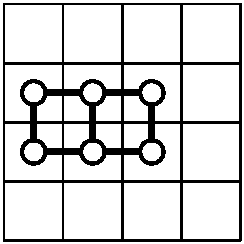
\includegraphics[width=0.9cm]{figures/NTuple-61.pdf}
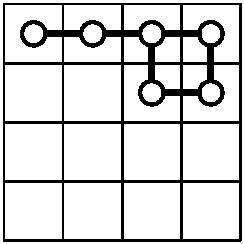
\includegraphics[width=0.9cm]{figures/NTuple-62.pdf}
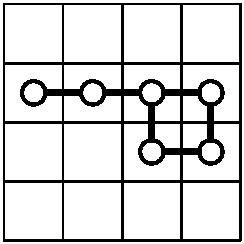
\includegraphics[width=0.9cm]{figures/NTuple-63.pdf}
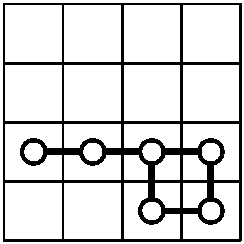
\includegraphics[width=0.9cm]{figures/NTuple-64.pdf}
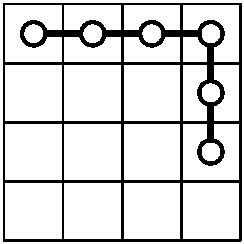
\includegraphics[width=0.9cm]{figures/NTuple-65.pdf}
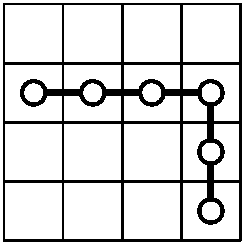
\includegraphics[width=0.9cm]{figures/NTuple-66.pdf}
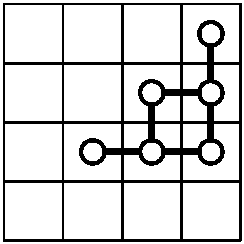
\includegraphics[width=0.9cm]{figures/NTuple-67.pdf}
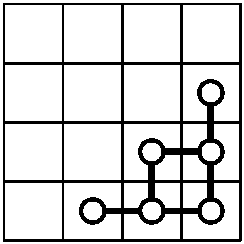
\includegraphics[width=0.9cm]{figures/NTuple-68.pdf}
& \raisebox{10pt}{$\begin{array}{r}
 \mbox{1 board, 2 stages}\\
612\,220\,032
 \end{array}$}
\\\hline
\raisebox{15pt}{\textsf{NT7}}
&
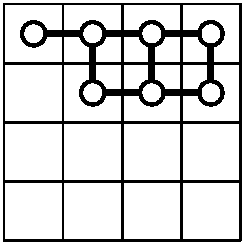
\includegraphics[width=0.9cm]{figures/NTuple-70.pdf}
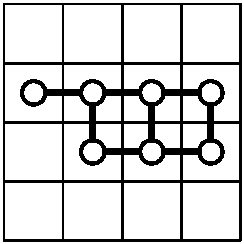
\includegraphics[width=0.9cm]{figures/NTuple-71.pdf}
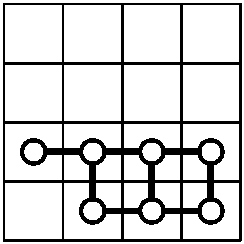
\includegraphics[width=0.9cm]{figures/NTuple-72.pdf}
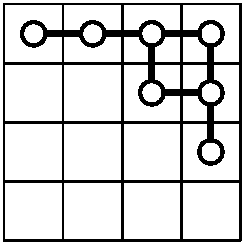
\includegraphics[width=0.9cm]{figures/NTuple-73.pdf}
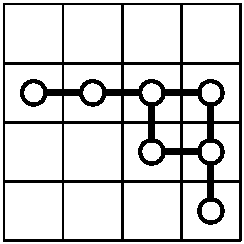
\includegraphics[width=0.9cm]{figures/NTuple-74.pdf}
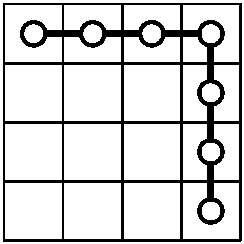
\includegraphics[width=0.9cm]{figures/NTuple-75.pdf}
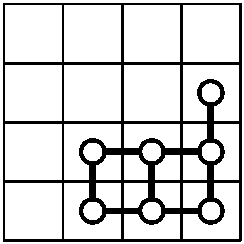
\includegraphics[width=0.9cm]{figures/NTuple-76.pdf}
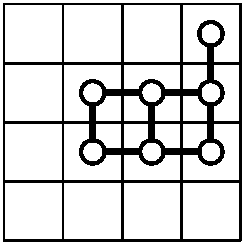
\includegraphics[width=0.9cm]{figures/NTuple-77.pdf}
& \raisebox{10pt}{$\begin{array}{r}
 \mbox{2 boards, 2 stages}\\
545\,640\,788
 \end{array}$}
\\\hline
\raisebox{15pt}{\textsf{NT8}}
&
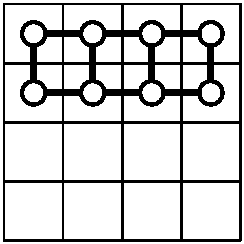
\includegraphics[width=0.9cm]{figures/NTuple-80.pdf}
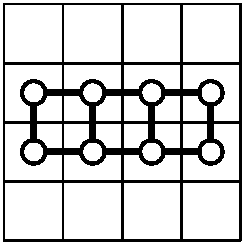
\includegraphics[width=0.9cm]{figures/NTuple-81.pdf}
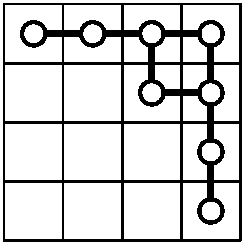
\includegraphics[width=0.9cm]{figures/NTuple-82.pdf}
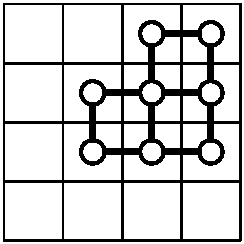
\includegraphics[width=0.9cm]{figures/NTuple-83.pdf}
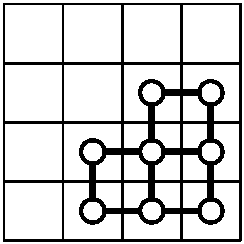
\includegraphics[width=0.9cm]{figures/NTuple-84.pdf}
& \raisebox{10pt}{$\begin{array}{r}
 \mbox{3 boards, 2 stages}\\
1\,291\,401\,630
 \end{array}$}
\\\hline
\raisebox{15pt}{\textsf{NT9}}
&
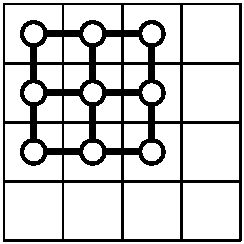
\includegraphics[width=0.9cm]{figures/NTuple-90.pdf}
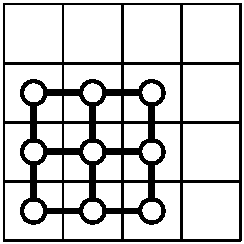
\includegraphics[width=0.9cm]{figures/NTuple-91.pdf}
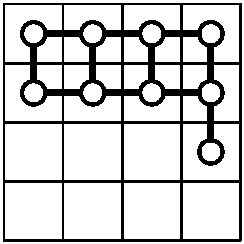
\includegraphics[width=0.9cm]{figures/NTuple-92.pdf}
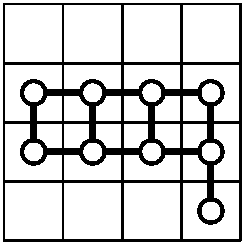
\includegraphics[width=0.9cm]{figures/NTuple-93.pdf}
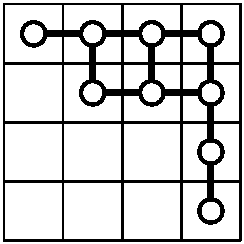
\includegraphics[width=0.9cm]{figures/NTuple-94.pdf}
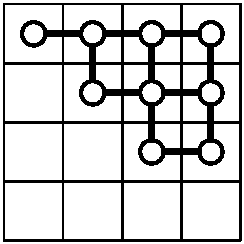
\includegraphics[width=0.9cm]{figures/NTuple-95.pdf}
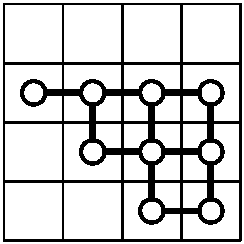
\includegraphics[width=0.9cm]{figures/NTuple-96.pdf}
& \raisebox{10pt}{$\begin{array}{r}
 \mbox{4 boards, 2 stages}\\
2\,259\,801\,992
 \end{array}$}
\\\hline
\end{tabular}
\end{table}

% 6G      NUM_TUPLES=8 NUM_SPLIT=1 で積は 48  メモリは  4.9GB (18^6*8*1*2*4*4)
% 6タプル NUM_TUPLES=9 NUM_SPLIT=1 で積は 54  メモリは  4.9GB (18^6*9*1*2*4*4)
% 7タプル NUM_TUPLES=7 NUM_SPLIT=2 で積は 98  メモリは  8.8GB (11^7*7*2*2*4*4)
% 8タプル NUM_TUPLES=5 NUM_SPLIT=3 で積は 120 メモリは 20.7GB ( 9^8*5*3*2*4*4)
% 9タプル NUM_TUPLES=7 NUM_SPLIT=4 で積は 252 メモリは 36.2GB ( 7^9*7*4*2*4*4)

\section{Experiments for 2048}

\subsection{Design of N-tuple Networks and Vertical Split Encoding}

% 6, 7, 8, 9 タプルをデザインした.デザインにあたっては,「妥当そうに見える形を人手で設計し,それらを平行移動する」ヒューリスティクスを用いた.
% 6タプル NT6 では,4つの形を選定し,それらを平行移動してできる9つの組合せとした.
% 7タプル NT7 では,4つの形を選定し,それらを平行移動してできる8つの組合せとした.
% 8タプル NT8 では,3つの形を選定し,それらを平行移動してできる5つの組合せとした.
% 9タプル NT9 では,4つの形を選定し,それらを平行移動してできる7つの組合せとした.
% baseline として,先行研究で用いられていた 8x6-tuples からなるネットワーク NT6-M を用いる.

Table~\ref{fig:NTupleVSE} summarizes the design of N-tuple Networks and Vertical Split Encoding
used in our experiments for 2048.

By adopting the heuristics of ``manually creating reasonable shapes and generating their translations''~\cite{Jask18}, we designed new sets of N-tuple networks for 6-, 7-, 8-, and 9-tuple cases.
\begin{itemize}
\item NT6: For the 6-tuple networks, we selected four shapes and by their translations obtained nine tuples.
\item NT7: For the 7-tuple networks, we selected four shapes and by their translations obtained eight tuples.
\item NT8: For the 8-tuple networks, we selected three shapes and by their translations obtained five tuples.
\item NT9: For the 9-tuple networks, we selected four shapes and by their translations obtained seven tuples.
\end{itemize}
As a baseline, we used NT6-M, a network consisting of 8$\times$6-tuples, which was first selected by Matsuzaki~\cite{Mats16} and employed in the state-of-the-art agent by Guei et al.~\cite{GuCW22}.

% それぞれの N-Tuple について,各パラメータを 64 bits とし,3倍のメモリを必要とする TC 学習と,2倍のメモリを必要とする multi-staging を用いても64 GBメモリに収まることを要件として,VSE の value ranges を設計した.
% 6タプルからなる NT6 と NT6M の場合は VSE なしで十分メモリに収まる.
% 7タプルからなる NT7 の場合には,少なくとも 2 つに分ける必要があり,2つのvalue ranges の大きさが 11 + 10 となるように分けた.
% 8タプルからなる NT8 の場合には,少なくとも 3 つに分ける必要があり,3つのvalue ranges の大きさが 9 + 9 + 6 となるように分けた.
% 9タプルからなる NT9 の場合には,少なくとも 4 つに分ける必要があり,4つのvalue ranges の大きさが 7 + 7 + 7 + 6 となるように分けた.
For each set of N-tuples, we designed the VSE value ranges under the following assumptions: each element in lookup tables has 64 bits; we use temporal coherence learning~\cite{Jask18} that requires three times the memory with three lookup tables; and we use multi-staging technique that requires two times the memory with two stages; the whole training program should fit within 64 GB of memory.
Under these assumption, our design of VSE was as follows.
\begin{itemize}
\item For NT6 and NT6-M, the parameters sufficiently fits within the memory without VSE.
\item For NT7, at least two splits are required, and we diivded into two value ranges of sizes being 11 and 10.
\item For NT8, at least three splits are needed, and we divided into three value ranges of sizes being 9, 9, and 6.
\item For NT9, at least four splits are needed, and we divided into four value ranges of sizes being 7, 7, 7, and 6.
\end{itemize}

% VSE の value ranges の取り方はもう少し自由度がある.それらを網羅的に試すのは今後の課題である.
Note that there exist a few more flexibility in the choice of value ranges in VSE.
Exhaustively exploring those possibilities remains as future work.

\subsection{Training and Evaluation with Expectimax Search}

% 上のように定義した N-tuple networks に対し,強化学習によってパラメータを調整した.
% 学習には,Optimistic initialization ありの Temporal Coherence 学習を用いた.
% Temporal coherence 学習(TC 学習):学習率を自動的に調整する機能を備えた TD 学習であり、Jaśkowski によって初めて 2048 に導入された手法である。本研究における N タプルネットワークの学習では、効率的かつ安定的な収束のために TC 学習を採用した。
% Optimistic initialization(OI):学習初期段階での探索を広く行うために、重みをゼロではなく大きな値で初期化する手法である。本研究では、すべての afterstate の初期値が 320,000 となるように重みを初期化した。
% OI 以外には,Exploration は入れていない.局所最適にならないよう,TC 学習で学習率を決定するパラメータを初期化する.$50 x 10^9$ step ごと.
% また,先行研究にならって,ゲームの進行に応じて重みを参照するテーブルを切り替える multi-staging 手法を用いる。本研究では 2 ステージから構成し、タイル 32768 が生成される前後でネットワークを切り替える.

For the N-tuple networks defined above, we conducted reinforcement learning to tune their parameters.
In this study, we employed Temporal Coherence learning with Optimistic Initialization and Restart Strategy.
\begin{description}
 \item[Temporal Coherence learning] Temporal Coherence learning is a variant of TD learning that enables automatic adjustment of the learning rate, which was first introduced to 2048 by Ja\'skowski~\cite{Jask18}.  To keep the effect of the following Optimistic Initialization, we decayed the learning rate from 0.5.
 \item[Optimistic Initialization] Optimistic Initialization is a method of encouraging exploration in the training by initializing the parameters with large values.  In this study, we use the same initial values as Guei et al.~\cite{GuCW22}: we initialize the parameters such that all afterstates have values of 320\,000.
 \item[Restart Strategy] The games of 2048 are easy at the beginning but hard when the board is filled with large-numbered tiles.  To address this issue, we appied the Restart Strategy proposed by Matsuzaki~\cite{Mats17} with constant number 10 of restarts.
 \item[Multi-staging] Following prior work~\cite{GuCW22}, we also employed the multi-staging method~\cite{YWHC16}, in which the lookup tables are switched depending on game progression. In this study, we split the game into two stages, switching the lookup tables before and after the generation of a 32\,768 tile.
\end{description}
We introduced no additional exploration in the training apart from Optimistic Initialization.
To avoid convergence to local optima, we reset the parameters controling the learning rate in Temporal Coherence learning every $50 \times 10^9$ steps.

% 本研究における学習は,6,7,8,9のそれぞれのタプルと既存研究で用いたタプルの5種類についてそれぞれ$200 x 10^11$ step分学習を行う.$1x10^9$ ごとにパラメータを出力し,1-ply lookahead (Greedy) プレイ 10000 ゲームの平均得点をモニターした.
% なお,random 要素の対応として,5つの異なるseedを用いて学習を行い,そられの平均と標準偏差を求めた.
In this study, for each of five types of N-tuple networks above, we conducted the training for $200 \times 10^{11}$ steps.  During the training, we output the parameters every $1 \times 10^9$ steps and evaluate their performance using the average score of 10\,000 games under 1-ply lookahead (Greedy) play.
To mitigate the randomness, we conducted the training with five different random seeds, and report their means and standard deviations.

% 図 \ref{fig:exp2} にtraining curve を示す.
% $200x10^9$ steps 学習した最終結果の平均得点を見ると,NT8 > NT7 > NT9 > NT6 $\approx$ NT6-M となっている.
% NT8 の標準偏差がとても大きくなっているのは,2つのseedが平均得点約 40万,残りの3つが約 32万 と大きく異なったためである.これら悪い場合をとっていても,NT6 と NT6-M よりも高得点である.
% NT7 と NT9 については,NT6 と NT6-M からの差が標準偏差よりも十分に大きい.したがって,N-Tuple のサイズを大きくすることで有意に性能向上したと言える.
% 学習の経過についてより詳しく見ると,NT7 だけが他のネットワークと学習曲線の形が異なっている.
% NT7 の学習が他よりも遅かった理由について,タプルの形によるものか,2-VSE によるものか,現時点では分かっていない.
% また,もう一つ面白い点として,TC学習による学習率をリセットしたとき,タプルサイズが大きいもののほうがスコアの下がり方が小さい.
Figure~\ref{fig:exp2} shows the training curves.
The final average scores after the training with $200 \times 10^9$ steps were ranked as NT8 $>$ NT7 $>$ NT9 $>$ NT6 $\approx$ NT6-M.
The standard deviation of NT8 was very large because tranining with two seeds succeeded achieving average scores of around 400\,000, while training with the other three saturated at around 320\,000.
Even considering these poor cases, NT8 still outperformed NT6 and NT6-M.
For NT7 and NT9, the differences from NT6 and NT6-M were sufficiently larger than their standard deviations.
These results indicate that increasing the N-tuple size significantly improved performance.

A closer look at the training progress reveals that when the learning rates were reset in Temporal Coherence learning, networks with larger tuple sizes showed smaller drops in score. This means that the training could be more stable with larger tuple sizes but at the same time they tend to converge local optima.
Another interesting observation is that NT7 was the only networks with a learning curve with a different shape.  Possible reasons for that slower learning would be its tuple design or the use of 2-VSE, but we have no clear evidences so far.

\begin{figure}
 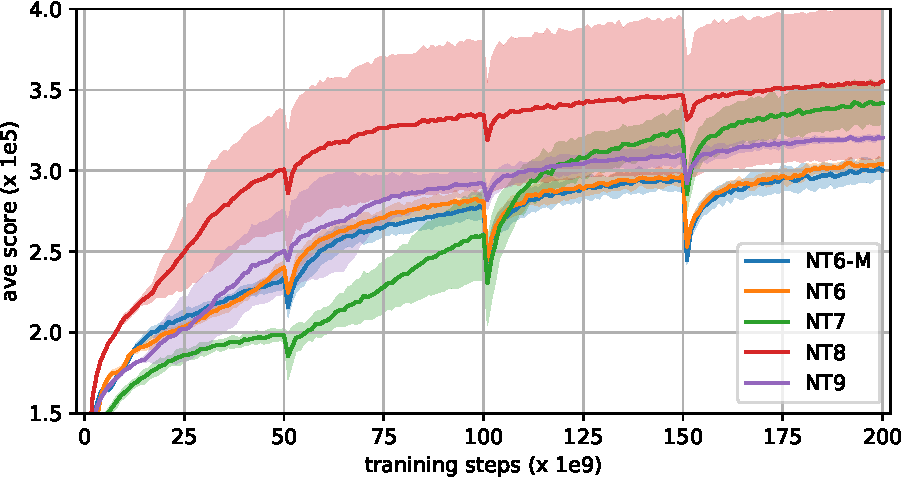
\includegraphics[width=.95\linewidth]{figures/plot-exp2.pdf}
 \caption{Training curve evaluated with 10000 games of the greedy play. The shaded areas show the standard deviations from five training runs.}
 \label{fig:exp2}
\end{figure}

% 最終的に得られたN-tuple network を用いて,Expectimax 探索 (3-ply, 5-ply) と組合せた評価も行った.
% 結果を \ref{table:exp3} に示す.
% 平均得点だけを見ると,3-ply や 5-ply のExpectimax探索を組み合わせたときに,NT6 や NT6-M を超える平均得点
% だったのは NT7 だけである.NT9 では,探索を組み合わせてもほとんど性能向上がない.
% とくに,32768 のタイルの生成率がすべて 0.0 \% となってしまっている.
% これは,lookup table のパラメータ数が多すぎるため局所最適な解へと学習してしまったことが原因と思われる.
% NT8 についても,学習がうまくいって1-ply で平均40万点であるものはExpectimax 探索で性能向上しているものの,
% 学習が停滞したものについては NT9 と同様に32768タイルの到達に失敗してしまっている.
% これにより,平均得点および32768タイルの到達率それぞれ標準偏差が非常に大きい結果となっている.
We also evaluated the final N-tuple networks in combination with Expectimax search (3-ply and 5-ply).
The results are shown in Table~\ref{table:exp3}.

Looking only at the average scores when combined with 3-ply or 5-ply Expectimax search, NT7 was the only network that outperformed NT6 and NT6-M.
For NT9, the addition of search provided almost no improvement in performance. In fact, the generation rate of the 32\,768 tile was 0.0\% in all cases. This is likely due to overfitting: the lookup table contained too many parameters, causing the network to converge to local optima that fail to reach a 32\,768 tile.
For NT8, if training was successful (achieving around 400\,000 points in 1-ply play), the combination of Expectimax search further improved performance. However, when training saturated, NT8 exhibited behavior similar to NT9, failing to reach a 32\,768 tile. As a result, both the average score and the 32\,768-tile reaching rate showed very large standard deviations.

\begin{table}
 \caption{Experiment results}
 \label{table:exp3}
 \small\begin{tabular}{l|l|l|l|l|l|l|l|l|l}
  \hline \hline
  & \multicolumn{2}{c}{1-ply (10000 games)} & \multicolumn{2}{c}{3-ply (1000 games)} & \multicolumn{2}{c}{5-ply (100 games)} \\
  & ave. score & 32768[\%] & ave. score & 32768[\%] & ave. score & 32768[\%] \\
  \hline
   NT0 (no VSE) & 300241$\pm$\phantom{0}5922	& 14.3$\pm$\phantom{0}1.7		& 462677$\pm$15573		& 44.3$\pm$\phantom{0}4.7		& 508618$\pm$\phantom{0}15010	& 55.0$\pm$\phantom{0}4.9 \\ \hline
   NT6 (no VSE) & 304149$\pm$\phantom{0}4361	& 14.9$\pm$\phantom{0}0.4		& 481544$\pm$\phantom{0}5497	& 47.8$\pm$\phantom{0}0.4	& 533801$\pm$\phantom{0}18084	& 61.3$\pm$\phantom{0}5.0 \\ \hline
   NT7 (2-VSE)	& 342009$\pm$12427		& 19.1$\pm$\phantom{0}2.9		& 491425$\pm$19140		& 46.1$\pm$\phantom{0}5.1		& 550848$\pm$\phantom{0}19390	& 60.5$\pm$\phantom{0}5.1 \\\hline
   NT8 (3-VSE)	& 355420$\pm$47102		& 15.5$\pm$15.6				& 438702$\pm$91280		& 29.1$\pm$29.1		& 448579$\pm$102127	& 31.5$\pm$32.0 \\\hline
   NT9 (4-VSE)	& 320205$\pm$\phantom{0}1404	& \phantom{0}0.0$\pm$\phantom{0}0.0	& 360286$\pm$\phantom{0}1446	& \phantom{0}0.0$\pm$\phantom{0}0.0		& 363160$\pm$\phantom{00}1886	& \phantom{0}0.0$\pm$\phantom{0}0.0 \\\hline
 \end{tabular}
\end{table}

\subsection{Evaluation of Best N-tuple Networks}

% 特に,NT8 で学習がうまくいったものとうまくいかなかったものがあったので,局所最適に陥いってしまったNT9を除くそれぞれのN-Tupleの大きさについて,5つの学習のうちもっともうまくいったネットワークを用いての評価を行った.
% 1つのネットワークに対して,5つの異なるシードでテストプレイ (1-ply, 3-ply, 5-ply) を行った結果を表 \ref{table:exp4} に示す.

% best ネットワークを用いた結果では,NT8 > NT7 > NT6 $\approx$ NT6-M となった.
% 5-ply の探索を組み合わせた場合についても,NT8 と NT6-M との差は7万点と標準偏差と比べて十分に大きな差が得られいる.
% したがって,VSE を組合せることでタプルサイズを大きくすることは,非常に有効だと結論付ける.

Since NT8, in particular, produced both successful and unsuccessful training outcomes, we conducted an additional evaluation using the best-performing networks for each N-tuple size, excluding NT9.
For each selected network, we ran test plays (10\,000 games with 1-ply lookahead, 1\,000 games with 3-ply, and 100 games with 5-ply) with five different random seeds.
The results are summarized in Table \ref{table:exp4}.

Using the best networks, the overall ranking was again NT8 $>$ NT7 $>$ NT6 $\approx$ NT6-M.
For the case combined with 5-ply Expectimax search, the performance gap between NT8 and NT6-M was about 70\,000, which is sufficiently larger than the standard deviation.
These results lead us to conclude that combining VSE with larger tuple sizes is highly effective for 2048.

\begin{table}
 \caption{Results of best agents}
 \label{table:exp4}
 \small\begin{tabular}{l|l|l|l|l|l|l|l|l|l}
  \hline \hline
  & \multicolumn{2}{c}{1-ply (10000 games)} & \multicolumn{2}{c}{3-ply (1000 games)} & \multicolumn{2}{c}{5-ply (100 games)} \\
  & ave. score & 32768[\%] & ave. score & 32768[\%] & ave. score & 32768[\%] \\
  \hline
   best NT0 (no VSE)	& 311\,354$\pm$1\,971		& 16.9$\pm$0.3	& 484\,281$\pm$5\,435	& 49.0$\pm$1.2	& 517\,595$\pm$17\,160	& 56.2$\pm$5.7 \\\hline
   best NT6 (no VSE)	& 300\,410$\pm$1\,122		& 14.4$\pm$0.4	& 484\,718$\pm$6\,182	& 48.1$\pm$1.0	& 532\,599$\pm$28\,947	& 58.4$\pm$8.5 \\\hline
   best NT7 (2-VSE)	& 341\,636$\pm$1\,719		& 19.0$\pm$0.2	& 484\,328$\pm$6\,187	& 44.2$\pm$1.9	& 541\,210$\pm$22\,938	& 56.6$\pm$5.8 \\\hline
   best NT8 (3-VSE)	& 407\,206$\pm$\phantom{1\,}432 & 30.0$\pm$0.2	& 547\,365$\pm$4\,938	& 57.2$\pm$1.9	& 587\,690$\pm$20\,439	& 66.2$\pm$6.2 \\\hline
 \end{tabular}
\end{table}

% \section{Consideration}
\section{Conclusion}
% 本研究では,2048 における強力なNタプルネットワークの設計に関する課題に取り組んだ。
% Nタプルネットワークは一般に,タプルのサイズを大きくするほど表現力が増し,性能の向上が期待できる。
% しかし同時に,タプルのサイズを大きくするたびにパラメータ数が指数的に増加し,必要なメモリと学習時間が膨大になるという深刻な問題を抱えていた.そのため,commodity computer で扱えるタプルサイズは6 または 7 が上限であった.
% この問題を解決するために,本研究では新しい符号化手法である Vertical Split Encoding (VSE) を提案した。
In this study, we have proposed a novel approach to designing powerful N-tuple networks for the game 2048.
Increasing the tuple size of N-tuple networks is expected to enhance the players' performance.
However, this comes with the severe drawback that the number of parameters and memory requirement grow exponentially with tuple size.  As a result, on commodity computers, the practical upper limit on tuple size had been restricted to six or seven for the game 2048.
To break through this limitation, we proposed a novel method called Vertical Split Encoding (VSE).

% まずMini2048 を用いた予備実験により,VSE を適用しても性能を大きく損なうことがないことを確認した.
% 次に,6タプル,7タプル(2-VSE),8タプル(3-VSE),9タプル(4-VSE)のネットワークを用いて2048のプレイヤを構築し,学習と評価を行った。
% その結果,VSE を適用することで新しく実現できたNタプルネットワークはいずれも6タプルのベースラインを上回った。
% 特に 8タプル+3-VSE は,5-ply Expectimax 探索で 594,619 という高いスコアを達成した。SOTAプレイヤで用いられていたNT6-M との同条件での比較で約70,000点の差となり,これは標準偏差を十分に上回る有意な差であった。
% これにより,VSE が大規模 Nタプルネットワークの性能を引き出す有効な手法であることを示した。

A preliminary experiment using Mini2048 confirmed that applying VSE does not cause substantial performance degradation.
We then built and trained 2048 players using N-tuple networks of tuple size six (\textsf{NT6} without VSE), seven (\textsf{NT7} with 2-VSE), eight (\textsf{NT8} with 3-VSE), and nine (\textsf{NT9} with 4-VSE).
The training results showed that all of \textsf{NT7}, \textsf{NT8}, and \textsf{NT9} networks outperformed the baseline (\textsf{NT6-M}).
In particular, the best player developed with \textsf{NT8} and 3-VSE achieved a high score of 587\,690 with 5-ply Expectimax search. Compared under the same conditions, this was about 70\,000 points higher than that of \textsf{NT6-M}, the network employed in the state-of-the-art player, and the improvement was far exceeding the standard deviation.
These findings demonstrate that VSE enables the design of N-tuple networks with larger tuple sizes and accordingly improvement of players.

% 今後の課題として,まず VSE を用いた大きなN-tuple Networksの設計は今回手作業および経験則に基づいている.
% 実験において,NT7 (3-VSE) の学習が遅いことなど,今回の設計には最適化の余地がありそうである.
% また,大規模タプルネットワーク,特に NT8 以上では学習が局所最適に陥っているという課題が残っている.
% これについては,学習率の制御方法やExploration の導入方法による改善を試みることが今後の取り組みである.
% これらの改良により,現在の SOTA プレイヤの平均得点 625900 を超えることが我々のゴールである.
Our future work includes the optimization of the design of large N-tuple networks with VSE, instead of manual heuristics and empirical choices.
Our experiments suggested that there is room for optimization: for example, the slower learning curve observed for \textsf{NT7} with 2-VSE.
Another important future work is to address the issue of performance plateau that was seen for NT9.
The improvement of learning-rate control and the introduction of exploration strategies during the training will be an important next step.
Our ultimate goal is to surpass the current state-of-the-art average score of 625\,377 with these improvements.


% 本研究の主な貢献は三点にまとめられる。第一に,従来はメモリや学習時間の制約から現実的に扱うことが困難であった大規模タプルを,VSE を用いることで実用的に利用可能にした点である。
% 第二に,提案手法を用いた大規模Nタプルネットワークが,従来最先端であった6タプルベースのプレイヤを上回る性能を示すことを実験的に確認した点である。
% 第三に,Nタプルネットワーク研究において「表現力を維持しつつパラメータを効率化する」という新しい方向性を提示した点である。

% LocalWords:  approximators VSE


\bibliographystyle{splncs04}
\bibliography{ref}

\end{document}

\begin{credits}
\subsubsection{\ackname} A bold run-in heading in small font size at the end of the paper is
used for general acknowledgments, for example: This study was funded
by X (grant number Y).

\subsubsection{\discintname}
It is now necessary to declare any competing interests or to specifically
state that the authors have no competing interests. Please place the
statement with a bold run-in heading in small font size beneath the
(optional) acknowledgments\footnote{If EquinOCS, our proceedings submission
system, is used, then the disclaimer can be provided directly in the system.},
for example: The authors have no competing interests to declare that are
relevant to the content of this article. Or: Author A has received research
grants from Company W. Author B has received a speaker honorarium from
Company X and owns stock in Company Y. Author C is a member of committee Z.
\end{credits}
%
% ---- Bibliography ----
%
% BibTeX users should specify bibliography style 'splncs04'.
% References will then be sorted and formatted in the correct style.
%
% \bibliographystyle{splncs04}
% \bibliography{mybibliography}
%
\begin{thebibliography}{8}
\bibitem{ref_article1}
Author, F.: Article title. Journal \textbf{2}(5), 99--110 (2016)

\bibitem{ref_lncs1}
Author, F., Author, S.: Title of a proceedings paper. In: Editor,
F., Editor, S. (eds.) CONFERENCE 2016, LNCS, vol. 9999, pp. 1--13.
Springer, Heidelberg (2016). \doi{10.10007/1234567890}

\bibitem{ref_book1}
Author, F., Author, S., Author, T.: Book title. 2nd edn. Publisher,
Location (1999)

\bibitem{ref_proc1}
Author, A.-B.: Contribution title. In: 9th International Proceedings
on Proceedings, pp. 1--2. Publisher, Location (2010)

\bibitem{ref_url1}
LNCS Homepage, \url{http://www.springer.com/lncs}, last accessed 2023/10/25
\end{thebibliography}
